% Options for packages loaded elsewhere
\PassOptionsToPackage{unicode}{hyperref}
\PassOptionsToPackage{hyphens}{url}
%
\documentclass[
]{article}
\usepackage{amsmath,amssymb}
\usepackage{lmodern}
\usepackage{ifxetex,ifluatex}
\ifnum 0\ifxetex 1\fi\ifluatex 1\fi=0 % if pdftex
  \usepackage[T1]{fontenc}
  \usepackage[utf8]{inputenc}
  \usepackage{textcomp} % provide euro and other symbols
\else % if luatex or xetex
  \usepackage{unicode-math}
  \defaultfontfeatures{Scale=MatchLowercase}
  \defaultfontfeatures[\rmfamily]{Ligatures=TeX,Scale=1}
\fi
% Use upquote if available, for straight quotes in verbatim environments
\IfFileExists{upquote.sty}{\usepackage{upquote}}{}
\IfFileExists{microtype.sty}{% use microtype if available
  \usepackage[]{microtype}
  \UseMicrotypeSet[protrusion]{basicmath} % disable protrusion for tt fonts
}{}
\makeatletter
\@ifundefined{KOMAClassName}{% if non-KOMA class
  \IfFileExists{parskip.sty}{%
    \usepackage{parskip}
  }{% else
    \setlength{\parindent}{0pt}
    \setlength{\parskip}{6pt plus 2pt minus 1pt}}
}{% if KOMA class
  \KOMAoptions{parskip=half}}
\makeatother
\usepackage{xcolor}
\IfFileExists{xurl.sty}{\usepackage{xurl}}{} % add URL line breaks if available
\IfFileExists{bookmark.sty}{\usepackage{bookmark}}{\usepackage{hyperref}}
\hypersetup{
  pdftitle={20220404\_miss\_data\_model},
  hidelinks,
  pdfcreator={LaTeX via pandoc}}
\urlstyle{same} % disable monospaced font for URLs
\usepackage[margin=1in]{geometry}
\usepackage{color}
\usepackage{fancyvrb}
\newcommand{\VerbBar}{|}
\newcommand{\VERB}{\Verb[commandchars=\\\{\}]}
\DefineVerbatimEnvironment{Highlighting}{Verbatim}{commandchars=\\\{\}}
% Add ',fontsize=\small' for more characters per line
\usepackage{framed}
\definecolor{shadecolor}{RGB}{248,248,248}
\newenvironment{Shaded}{\begin{snugshade}}{\end{snugshade}}
\newcommand{\AlertTok}[1]{\textcolor[rgb]{0.94,0.16,0.16}{#1}}
\newcommand{\AnnotationTok}[1]{\textcolor[rgb]{0.56,0.35,0.01}{\textbf{\textit{#1}}}}
\newcommand{\AttributeTok}[1]{\textcolor[rgb]{0.77,0.63,0.00}{#1}}
\newcommand{\BaseNTok}[1]{\textcolor[rgb]{0.00,0.00,0.81}{#1}}
\newcommand{\BuiltInTok}[1]{#1}
\newcommand{\CharTok}[1]{\textcolor[rgb]{0.31,0.60,0.02}{#1}}
\newcommand{\CommentTok}[1]{\textcolor[rgb]{0.56,0.35,0.01}{\textit{#1}}}
\newcommand{\CommentVarTok}[1]{\textcolor[rgb]{0.56,0.35,0.01}{\textbf{\textit{#1}}}}
\newcommand{\ConstantTok}[1]{\textcolor[rgb]{0.00,0.00,0.00}{#1}}
\newcommand{\ControlFlowTok}[1]{\textcolor[rgb]{0.13,0.29,0.53}{\textbf{#1}}}
\newcommand{\DataTypeTok}[1]{\textcolor[rgb]{0.13,0.29,0.53}{#1}}
\newcommand{\DecValTok}[1]{\textcolor[rgb]{0.00,0.00,0.81}{#1}}
\newcommand{\DocumentationTok}[1]{\textcolor[rgb]{0.56,0.35,0.01}{\textbf{\textit{#1}}}}
\newcommand{\ErrorTok}[1]{\textcolor[rgb]{0.64,0.00,0.00}{\textbf{#1}}}
\newcommand{\ExtensionTok}[1]{#1}
\newcommand{\FloatTok}[1]{\textcolor[rgb]{0.00,0.00,0.81}{#1}}
\newcommand{\FunctionTok}[1]{\textcolor[rgb]{0.00,0.00,0.00}{#1}}
\newcommand{\ImportTok}[1]{#1}
\newcommand{\InformationTok}[1]{\textcolor[rgb]{0.56,0.35,0.01}{\textbf{\textit{#1}}}}
\newcommand{\KeywordTok}[1]{\textcolor[rgb]{0.13,0.29,0.53}{\textbf{#1}}}
\newcommand{\NormalTok}[1]{#1}
\newcommand{\OperatorTok}[1]{\textcolor[rgb]{0.81,0.36,0.00}{\textbf{#1}}}
\newcommand{\OtherTok}[1]{\textcolor[rgb]{0.56,0.35,0.01}{#1}}
\newcommand{\PreprocessorTok}[1]{\textcolor[rgb]{0.56,0.35,0.01}{\textit{#1}}}
\newcommand{\RegionMarkerTok}[1]{#1}
\newcommand{\SpecialCharTok}[1]{\textcolor[rgb]{0.00,0.00,0.00}{#1}}
\newcommand{\SpecialStringTok}[1]{\textcolor[rgb]{0.31,0.60,0.02}{#1}}
\newcommand{\StringTok}[1]{\textcolor[rgb]{0.31,0.60,0.02}{#1}}
\newcommand{\VariableTok}[1]{\textcolor[rgb]{0.00,0.00,0.00}{#1}}
\newcommand{\VerbatimStringTok}[1]{\textcolor[rgb]{0.31,0.60,0.02}{#1}}
\newcommand{\WarningTok}[1]{\textcolor[rgb]{0.56,0.35,0.01}{\textbf{\textit{#1}}}}
\usepackage{graphicx}
\makeatletter
\def\maxwidth{\ifdim\Gin@nat@width>\linewidth\linewidth\else\Gin@nat@width\fi}
\def\maxheight{\ifdim\Gin@nat@height>\textheight\textheight\else\Gin@nat@height\fi}
\makeatother
% Scale images if necessary, so that they will not overflow the page
% margins by default, and it is still possible to overwrite the defaults
% using explicit options in \includegraphics[width, height, ...]{}
\setkeys{Gin}{width=\maxwidth,height=\maxheight,keepaspectratio}
% Set default figure placement to htbp
\makeatletter
\def\fps@figure{htbp}
\makeatother
\setlength{\emergencystretch}{3em} % prevent overfull lines
\providecommand{\tightlist}{%
  \setlength{\itemsep}{0pt}\setlength{\parskip}{0pt}}
\setcounter{secnumdepth}{-\maxdimen} % remove section numbering
\ifluatex
  \usepackage{selnolig}  % disable illegal ligatures
\fi

\title{20220404\_miss\_data\_model}
\author{}
\date{\vspace{-2.5em}}

\begin{document}
\maketitle

I do \emph{not} know how to specify these missing data models.

Let's try anyways!

\begin{Shaded}
\begin{Highlighting}[]
\CommentTok{\# loading packages}
\FunctionTok{library}\NormalTok{(sna)}
\FunctionTok{library}\NormalTok{(ergm)}
\end{Highlighting}
\end{Shaded}

\hypertarget{generate-some-toy-networks}{%
\subsection{Generate some toy
networks}\label{generate-some-toy-networks}}

\begin{Shaded}
\begin{Highlighting}[]
\CommentTok{\# fix seed for now}
\FunctionTok{set.seed}\NormalTok{(}\DecValTok{123}\NormalTok{)}

\CommentTok{\# just generating a random graph}
\NormalTok{testNet }\OtherTok{=} \FunctionTok{rgraph}\NormalTok{(}\AttributeTok{n =} \DecValTok{20}\NormalTok{,}
                   \AttributeTok{m =} \DecValTok{1}\NormalTok{,}
                   \AttributeTok{tprob =} \FloatTok{0.5}\NormalTok{,}
                   \AttributeTok{mode =} \StringTok{"graph"}\NormalTok{)}

\CommentTok{\# number of ties}
\FunctionTok{sum}\NormalTok{(testNet)}
\end{Highlighting}
\end{Shaded}

\begin{verbatim}
## [1] 206
\end{verbatim}

\begin{Shaded}
\begin{Highlighting}[]
\CommentTok{\# since it\textquotesingle{}s symmetric (undirected), the unique ties are half of that sum.}
\end{Highlighting}
\end{Shaded}

\hypertarget{missing-completely-at-random}{%
\subsubsection{Missing completely at
random}\label{missing-completely-at-random}}

\begin{Shaded}
\begin{Highlighting}[]
\CommentTok{\# let\textquotesingle{}s do an MCAR example for comparison}
\NormalTok{missThresh }\OtherTok{=} \FunctionTok{matrix}\NormalTok{( }\AttributeTok{data =} \FunctionTok{runif}\NormalTok{(}\DecValTok{20}\SpecialCharTok{\^{}}\DecValTok{2}\NormalTok{, }\AttributeTok{min =} \DecValTok{0}\NormalTok{, }\AttributeTok{max =} \DecValTok{1}\NormalTok{),}
                     \AttributeTok{nrow =} \DecValTok{20}\NormalTok{,}
                     \AttributeTok{ncol =} \DecValTok{20}\NormalTok{ )}

\DocumentationTok{\#\# }\AlertTok{NOTE}\DocumentationTok{: for an undirected network, this needs to be symmetric so}
\CommentTok{\# overwrite the upper triangle with the lower triangle}
\NormalTok{missThresh[}\FunctionTok{upper.tri}\NormalTok{(missThresh)] }\OtherTok{=} \FunctionTok{t}\NormalTok{(missThresh)[}\FunctionTok{upper.tri}\NormalTok{(missThresh)]}

\CommentTok{\# set a proportion of missing entries, 0.2 would imply that 20\% of all tie variables are missing.}
\NormalTok{propMiss }\OtherTok{=} \FloatTok{0.2}

\CommentTok{\# index which tie variables are missing}
\NormalTok{missTieVars }\OtherTok{=}\NormalTok{ missThresh }\SpecialCharTok{\textless{}=}\NormalTok{ propMiss}

\CommentTok{\# degrade the network}
\NormalTok{degradedNet }\OtherTok{=}\NormalTok{ testNet}
\NormalTok{degradedNet[missTieVars] }\OtherTok{=} \ConstantTok{NA}

\CommentTok{\# check how many are missing (should be \textasciitilde{}propMiss * n\^{}2)}
\FunctionTok{sum}\NormalTok{(}\FunctionTok{is.na}\NormalTok{(degradedNet))}
\end{Highlighting}
\end{Shaded}

\begin{verbatim}
## [1] 83
\end{verbatim}

\begin{Shaded}
\begin{Highlighting}[]
\CommentTok{\# diagonal of 0}
\FunctionTok{diag}\NormalTok{(degradedNet) }\OtherTok{=} \DecValTok{0}

\CommentTok{\# plot side by side}
\FunctionTok{par}\NormalTok{(}\AttributeTok{mfrow =} \FunctionTok{c}\NormalTok{(}\DecValTok{1}\NormalTok{,}\DecValTok{2}\NormalTok{))}
\NormalTok{coord }\OtherTok{=} \FunctionTok{gplot}\NormalTok{(testNet, }\AttributeTok{xlab =} \StringTok{"Toy net"}\NormalTok{, }\AttributeTok{gmode =} \StringTok{"graph"}\NormalTok{)}
\FunctionTok{gplot}\NormalTok{(degradedNet, }\AttributeTok{xlab =} \StringTok{"Degraded net"}\NormalTok{, }\AttributeTok{gmode =} \StringTok{"graph"}\NormalTok{, }\AttributeTok{coord =}\NormalTok{ coord)}
\end{Highlighting}
\end{Shaded}

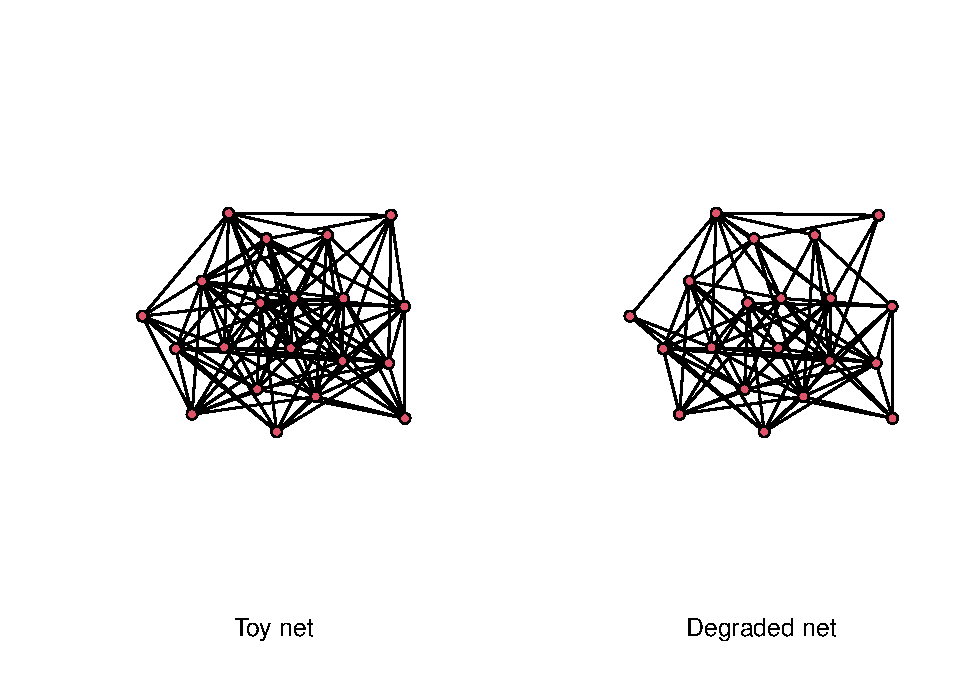
\includegraphics{20220404_miss_data_model_files/figure-latex/MCAR-1.pdf}

\begin{Shaded}
\begin{Highlighting}[]
\CommentTok{\# degree distributions}
\FunctionTok{hist}\NormalTok{(}\FunctionTok{degree}\NormalTok{(testNet), }\AttributeTok{main =} \FunctionTok{paste}\NormalTok{(}\StringTok{"Mean = "}\NormalTok{,}\FunctionTok{mean}\NormalTok{(}\FunctionTok{degree}\NormalTok{(testNet)), }\StringTok{" SD = "}\NormalTok{, }\FunctionTok{round}\NormalTok{(}\FunctionTok{sd}\NormalTok{(}\FunctionTok{degree}\NormalTok{(testNet)), }\DecValTok{2}\NormalTok{), }\AttributeTok{sep =} \StringTok{""}\NormalTok{))}
\FunctionTok{hist}\NormalTok{(}\FunctionTok{degree}\NormalTok{(degradedNet),}\AttributeTok{main =} \FunctionTok{paste}\NormalTok{(}\StringTok{"Mean = "}\NormalTok{,}\FunctionTok{mean}\NormalTok{(}\FunctionTok{degree}\NormalTok{(testNet)), }\StringTok{" SD = "}\NormalTok{, }\FunctionTok{round}\NormalTok{(}\FunctionTok{sd}\NormalTok{(}\FunctionTok{degree}\NormalTok{(degradedNet)), }\DecValTok{2}\NormalTok{), }\AttributeTok{sep =} \StringTok{""}\NormalTok{))}
\end{Highlighting}
\end{Shaded}

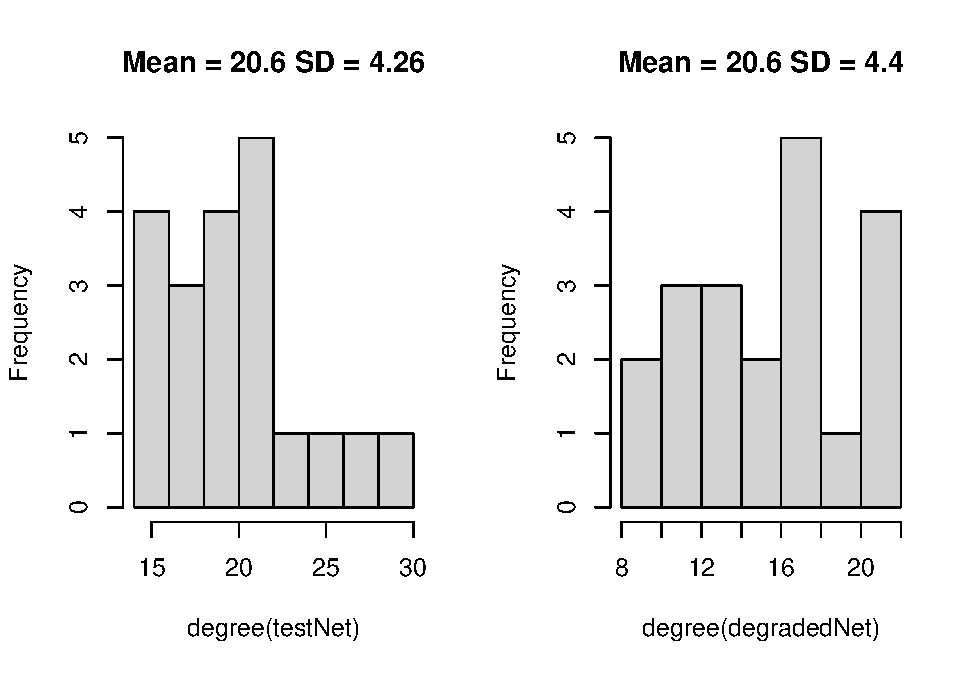
\includegraphics{20220404_miss_data_model_files/figure-latex/MCAR-2.pdf}

What's going on from the principles side of things?

This is basically saying:

\[\mathbf{D}|\mathbf{X} \sim Bern(\theta)\]

With \(\theta\) set to 0.2 in the example.

So, given the missing data model, we can then clarify how this is MCAR,

\[\Pr(\mathbf{D}|\mathbf{X}, \theta) = \Pr(\mathbf{D|\theta)} \text{ for all entries X and parameters } \theta .\]

So, the values in \(\mathbf{X}\) have absolutely no effect on how likely
a tie variable is in being missing.

Therefore, the data are missing completely at random (MCAR).

\hypertarget{missing-not-at-random}{%
\subsection{Missing not at random}\label{missing-not-at-random}}

Toy example: more central would imply more likely to be missing. From a
covert network perspective, this might be for security reasons. Another
perspective would be that because this particular figure is so central,
nobody nominates them because the nominators implicitly assumed this
central figure to already be acknowledged.

If we start by explaining the model,

\[\Pr(\mathbf{D}_{ij} = 1) = logistic(\alpha + \beta(\mathbf{X}_{i+} + \mathbf{X}_{+j}) )\]

Note that \(\mathbf{X}_{i+} + \mathbf{X}_{+j}\) is meant to reflect
degree (centrality). For the undirected case, this should be equivalent
to \(2 \times \mathbf{X}_{i+}\) or \(2 \times \mathbf{X}_{+j}\).

This needs to be set up in a way such that the higher the degree, the
more likely for the tie to be missing.

\begin{Shaded}
\begin{Highlighting}[]
\CommentTok{\# how to start..}

\CommentTok{\# make up some values for alpha and beta}
\NormalTok{alpha }\OtherTok{=} \SpecialCharTok{{-}}\DecValTok{5}  \CommentTok{\# an intercept value,}

\NormalTok{beta }\OtherTok{=} \FloatTok{0.17} \CommentTok{\# this beta value corresponds to the weight of the variable when assigning the probability of missingness}

\CommentTok{\# grab degrees}
\NormalTok{degCentr }\OtherTok{=} \FunctionTok{degree}\NormalTok{(testNet)}

\CommentTok{\# let\textquotesingle{}s figure out standardising this later...}
\CommentTok{\# maxDegree = 20*19}
\CommentTok{\# }
\CommentTok{\# \# normalise it with the maximum possible degree so scale is less of an issue (i.e., a form of standardisation)}
\CommentTok{\# normDegCentr = degCentr/maxDegree}
\CommentTok{\# }

\CommentTok{\# finalgle the probability such that the mean is \textasciitilde{}0.2}

\FunctionTok{mean}\NormalTok{(}\DecValTok{1}\SpecialCharTok{/}\NormalTok{(}\DecValTok{1} \SpecialCharTok{+} \FunctionTok{exp}\NormalTok{(}\SpecialCharTok{{-}}\NormalTok{alpha }\SpecialCharTok{{-}}\NormalTok{ (beta }\SpecialCharTok{*}\NormalTok{ degCentr))))}
\end{Highlighting}
\end{Shaded}

\begin{verbatim}
## [1] 0.2042103
\end{verbatim}

\begin{Shaded}
\begin{Highlighting}[]
\CommentTok{\# list out the probabilities}
\NormalTok{missTieProb }\OtherTok{=} \DecValTok{1}\SpecialCharTok{/}\NormalTok{(}\DecValTok{1} \SpecialCharTok{+} \FunctionTok{exp}\NormalTok{(}\SpecialCharTok{{-}}\NormalTok{alpha }\SpecialCharTok{{-}}\NormalTok{ (beta }\SpecialCharTok{*}\NormalTok{ degCentr)))}
\end{Highlighting}
\end{Shaded}

\textbf{Why did I pick these alpha and beta values?}

I started with trying to get an average missing tie variable probability
of \textasciitilde0.2 (similar to the MCAR example),

\[\frac{\sum_{i = 1..n} \frac{1}{1 + \exp(-\alpha -\mathbf{X}_i \beta)}}{n} = 0.2,\]

where \(\mathbf{X}_i\) here represents the (unnormalised) degree
centrality.

Also, working backwards,

\[1 + \exp(-\alpha - \mathbf{X}_i\beta) = 5,\]

\[\exp(-\alpha - \mathbf{X}_i\beta) = 4,\]

Let's use the mean degree in place of each individual to make life
easier,

\[\exp(-\alpha - \frac{\sum_{i = 1..n} \mathbf{X}_i}{n} \beta) = 4.\]

Let's use the selected random graph mean degree so
\(\frac{\sum_{i = 1..n} \mathbf{X}_i}{n} = 20.6\)

\[\exp(-\alpha - 20.6\beta) = 4,\]

\[-\alpha - 20.6\beta = \log(4),\]

\[\beta = \frac{-\log(4) - \alpha}{20.6}.\]

Let's graph that\ldots{}

\begin{Shaded}
\begin{Highlighting}[]
\CommentTok{\# make up some alpha values}
\NormalTok{alphaVal }\OtherTok{=} \FunctionTok{seq}\NormalTok{(}\AttributeTok{from =} \SpecialCharTok{{-}}\DecValTok{10}\NormalTok{, }\AttributeTok{to =} \DecValTok{10}\NormalTok{, }\AttributeTok{by =} \DecValTok{1}\NormalTok{)}

\NormalTok{betaVal }\OtherTok{=}\NormalTok{ (}\SpecialCharTok{{-}}\FunctionTok{log}\NormalTok{(}\DecValTok{4}\NormalTok{) }\SpecialCharTok{{-}}\NormalTok{ alphaVal)}\SpecialCharTok{/}\FloatTok{20.6}

\FunctionTok{plot}\NormalTok{(}\AttributeTok{x =}\NormalTok{ alphaVal, }\AttributeTok{y =}\NormalTok{ betaVal)}
\end{Highlighting}
\end{Shaded}

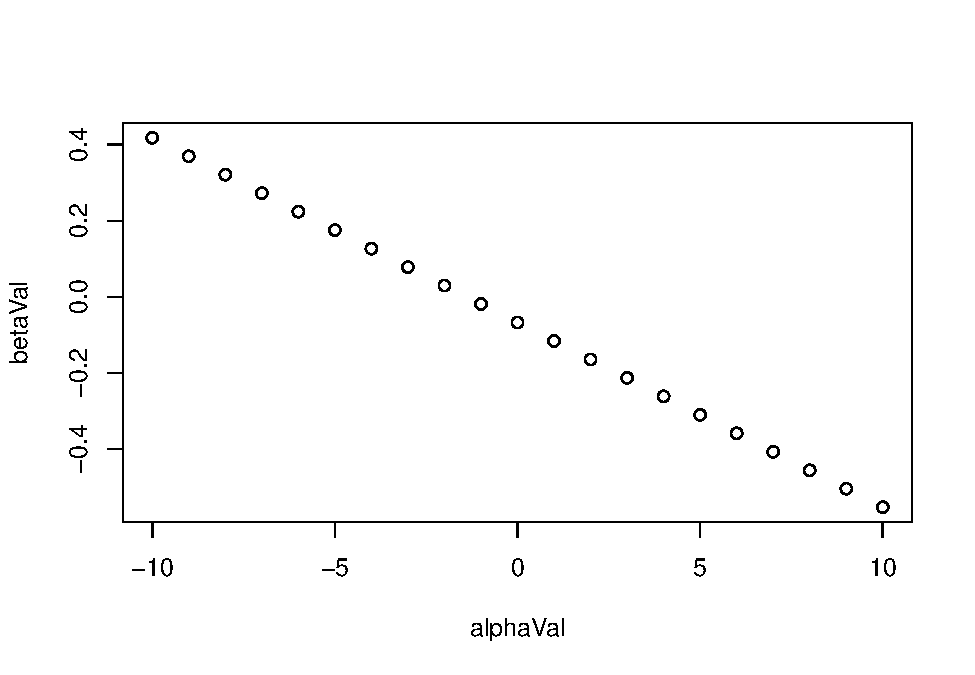
\includegraphics{20220404_miss_data_model_files/figure-latex/graphing fn-1.pdf}

Any pair of values here can be used, but we want \(\beta\) to have
certain properties,

\begin{itemize}
\tightlist
\item
  The absolute value of beta describes how much weight the variable in
  question affects the missing probability,\\
\item
  The sign of beta describes the relationship between the variable in
  question and the missing probability.
\end{itemize}

Our variable in question here is degree centrality, we want it to have a
pronounced effect, but not \emph{too} extreme. We also want beta's sign
to be positive to reflect a positive linear relationship between degree
centrality and the probability of a missing tie variable.

Hence we ended up with:

\[\alpha = -5 \\ \beta = 0.17\]

Now, apply that to the network degradation,

\begin{Shaded}
\begin{Highlighting}[]
\CommentTok{\# another seed because randomness.}
\FunctionTok{set.seed}\NormalTok{(}\DecValTok{132}\NormalTok{)}

\CommentTok{\# similar to the previous depletion,}
\CommentTok{\# we have a set of model{-}predicted missing tie probabilities}

\CommentTok{\# let\textquotesingle{}s first make a matrix of missing data indicators with the probabilities we have}
\CommentTok{\# the rbinom function\textquotesingle{}s just a convenient way of doing this, also each actor technically has an implicit \textasciitilde{}Bi(n, miss tie prob) amount of missing ties}
\NormalTok{missDatIndicator }\OtherTok{=} \FunctionTok{t}\NormalTok{(}\FunctionTok{replicate}\NormalTok{(}\DecValTok{20}\NormalTok{, }\FunctionTok{rbinom}\NormalTok{(}\FunctionTok{length}\NormalTok{(missTieProb), }\AttributeTok{size =} \DecValTok{1}\NormalTok{, }\AttributeTok{prob =}\NormalTok{ missTieProb)))}

\CommentTok{\# check how many were indicated to be missing}
\FunctionTok{sum}\NormalTok{(missDatIndicator)}
\end{Highlighting}
\end{Shaded}

\begin{verbatim}
## [1] 85
\end{verbatim}

\begin{Shaded}
\begin{Highlighting}[]
\CommentTok{\# make some adjustments because undirected network}
\NormalTok{missDatIndicator[}\FunctionTok{upper.tri}\NormalTok{(missDatIndicator)] }\OtherTok{=} \FunctionTok{t}\NormalTok{(missDatIndicator)[}\FunctionTok{upper.tri}\NormalTok{(missDatIndicator)]}
\FunctionTok{diag}\NormalTok{(missDatIndicator) }\OtherTok{=} \DecValTok{0}
\FunctionTok{isSymmetric}\NormalTok{(missDatIndicator)}
\end{Highlighting}
\end{Shaded}

\begin{verbatim}
## [1] TRUE
\end{verbatim}

\begin{Shaded}
\begin{Highlighting}[]
\CommentTok{\# make a table to compare,}
\NormalTok{compareTab }\OtherTok{=} \FunctionTok{data.frame}\NormalTok{(}\AttributeTok{missTieProb =} \FunctionTok{round}\NormalTok{(missTieProb, }\AttributeTok{digits =} \DecValTok{2}\NormalTok{), }\AttributeTok{IndicatorProbabilities =} \FunctionTok{colMeans}\NormalTok{(missDatIndicator))}
\NormalTok{compareTab}\SpecialCharTok{$}\NormalTok{difference }\OtherTok{=}\NormalTok{ compareTab[,}\DecValTok{1}\NormalTok{] }\SpecialCharTok{{-}}\NormalTok{ compareTab[,}\DecValTok{2}\NormalTok{]}
\FunctionTok{print}\NormalTok{(compareTab)}
\end{Highlighting}
\end{Shaded}

\begin{verbatim}
##    missTieProb IndicatorProbabilities difference
## 1         0.07                   0.15      -0.08
## 2         0.17                   0.20      -0.03
## 3         0.22                   0.35      -0.13
## 4         0.22                   0.25      -0.03
## 5         0.09                   0.20      -0.11
## 6         0.22                   0.20       0.02
## 7         0.09                   0.20      -0.11
## 8         0.17                   0.15       0.02
## 9         0.13                   0.30      -0.17
## 10        0.17                   0.10       0.07
## 11        0.44                   0.35       0.09
## 12        0.28                   0.15       0.13
## 13        0.13                   0.10       0.03
## 14        0.22                   0.35      -0.13
## 15        0.13                   0.15      -0.02
## 16        0.52                   0.30       0.22
## 17        0.22                   0.25      -0.03
## 18        0.07                   0.05       0.02
## 19        0.36                   0.20       0.16
## 20        0.17                   0.20      -0.03
\end{verbatim}

\begin{Shaded}
\begin{Highlighting}[]
\CommentTok{\# check total amount of missing ties after the adjmat adjustments, should be \textasciitilde{}80 (20\^{}2 * 0.2), maybe a bit less because of the adjmat adjustments}
\FunctionTok{sum}\NormalTok{(missDatIndicator)}
\end{Highlighting}
\end{Shaded}

\begin{verbatim}
## [1] 84
\end{verbatim}

\begin{Shaded}
\begin{Highlighting}[]
\CommentTok{\# and we deplete}
\NormalTok{degradedNetMNAR }\OtherTok{=}\NormalTok{ testNet}
\NormalTok{degradedNetMNAR[missDatIndicator}\SpecialCharTok{==}\DecValTok{1}\NormalTok{] }\OtherTok{=} \ConstantTok{NA}

\CommentTok{\# plot side by side}
\FunctionTok{par}\NormalTok{(}\AttributeTok{mfrow =} \FunctionTok{c}\NormalTok{(}\DecValTok{1}\NormalTok{,}\DecValTok{2}\NormalTok{))}
\FunctionTok{gplot}\NormalTok{(testNet, }\AttributeTok{xlab =} \StringTok{"Toy net"}\NormalTok{, }\AttributeTok{gmode =} \StringTok{"graph"}\NormalTok{)}
\FunctionTok{gplot}\NormalTok{(degradedNetMNAR, }\AttributeTok{xlab =} \StringTok{"MNAR degraded net"}\NormalTok{, }\AttributeTok{gmode =} \StringTok{"graph"}\NormalTok{)}
\end{Highlighting}
\end{Shaded}

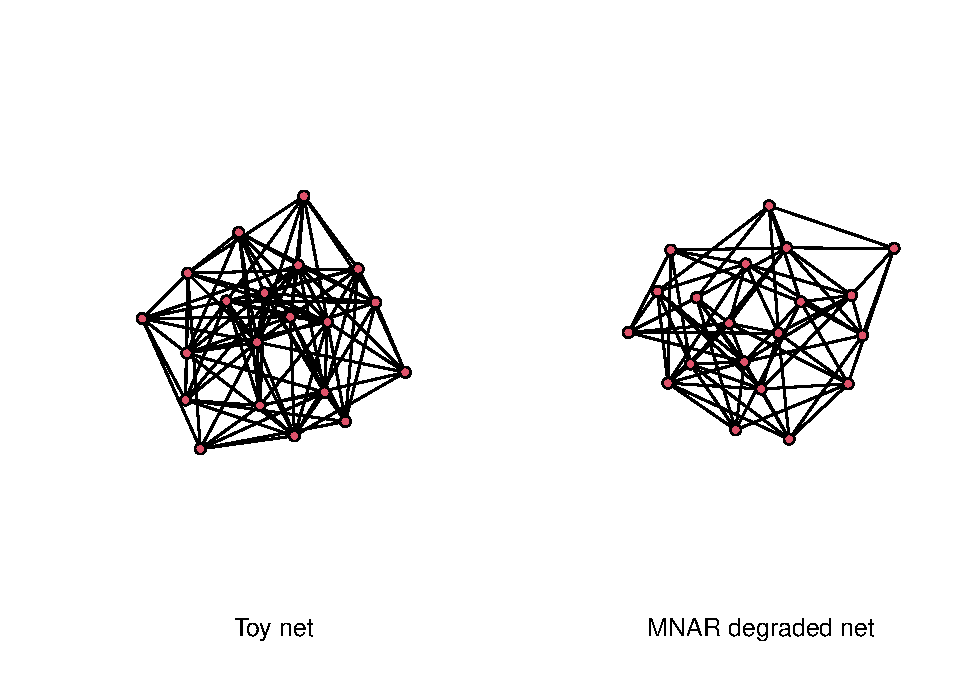
\includegraphics{20220404_miss_data_model_files/figure-latex/MNAR netdegrade-1.pdf}

\begin{Shaded}
\begin{Highlighting}[]
\CommentTok{\# it\textquotesingle{}s quite hard to see, but if we see the average degree centrality and their histograms,}
\FunctionTok{hist}\NormalTok{(}\FunctionTok{degree}\NormalTok{(testNet), }\AttributeTok{main =} \FunctionTok{paste}\NormalTok{(}\StringTok{"Mean = "}\NormalTok{,}\FunctionTok{mean}\NormalTok{(}\FunctionTok{degree}\NormalTok{(testNet)), }\StringTok{" SD = "}\NormalTok{, }\FunctionTok{round}\NormalTok{(}\FunctionTok{sd}\NormalTok{(}\FunctionTok{degree}\NormalTok{(testNet)), }\DecValTok{2}\NormalTok{), }\AttributeTok{sep =} \StringTok{""}\NormalTok{))}
\FunctionTok{hist}\NormalTok{(}\FunctionTok{degree}\NormalTok{(degradedNetMNAR), }\AttributeTok{main =} \FunctionTok{paste}\NormalTok{(}\StringTok{"Mean = "}\NormalTok{,}\FunctionTok{mean}\NormalTok{(}\FunctionTok{degree}\NormalTok{(degradedNetMNAR)), }\StringTok{" SD = "}\NormalTok{, }\FunctionTok{round}\NormalTok{(}\FunctionTok{sd}\NormalTok{(}\FunctionTok{degree}\NormalTok{(degradedNetMNAR)), }\DecValTok{2}\NormalTok{), }\AttributeTok{sep =} \StringTok{""}\NormalTok{))}
\end{Highlighting}
\end{Shaded}

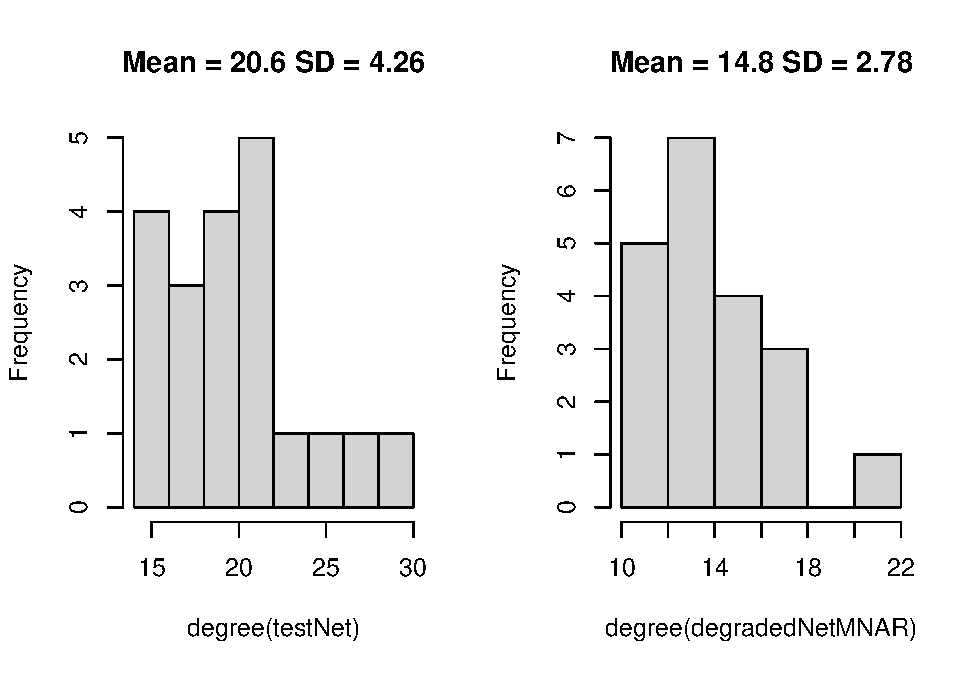
\includegraphics{20220404_miss_data_model_files/figure-latex/MNAR netdegrade-2.pdf}

\begin{Shaded}
\begin{Highlighting}[]
\CommentTok{\# the mean degree centrality may have decreased more? Hard to tell...}
\end{Highlighting}
\end{Shaded}

\textbf{What's going on with the MNAR depletion?}

First, we use a binomial distribution to generate missing tie variables
for each actor with the probability of a missing tie variable
corresponding to what we found out before with the missing data model.

So really,

\[\mathbf{D}| \mathbf{X}_{i} \sim Bi(n, p_i),\]

where the index \(i\) here refers to each actor with their own missing
tie variable probability which we modelled earlier (or the entire row),

\[\Pr(\mathbf{D}|\mathbf{X}_i) = logistic(\alpha + \beta \times (2 \times \mathbf{X}_{i+})),\]

which can also be written as:

\[p_i = logistic(\alpha + \beta \times (2 \times \mathbf{X}_{i+}).\]

Also reminder that \(2 \times \mathbf{X}_{i+}\) here just reflects an
actor's degree centralisation in this undirected network.

With that in mind, I made some manual adjustments so the adjacency
matrix makes sense (only 0s in the diagonal, symmetric for an undirected
network), and we now have a depleted network with a missing not at
random pattern of missingness.

\textbf{But why is it missing not at random and not the other two?}

As seen in the missing data model,

\[\Pr(\mathbf{D}|\mathbf{X}_i) = logistic(\alpha + \beta \times (2 \times \mathbf{X}_{i+})),\]

The fact that \(\mathbf{X}\) is there at all rules out MCAR.

The reason why this missing data model is not MAR is because of
\(\mathbf{X}_{i+}\) since this sum would need both the observed and
depleted tie variables,

\[\mathbf{X}_{i+} = \mathbf{X_{obs}}_{i+} +  \mathbf{X_{mis}}_{i+},\]

so conceptually,

\[\Pr(\mathbf{D}|\mathbf{X}, p) = \Pr(\mathbf{D} | \mathbf{X}_{obs}, \mathbf{X}_{mis}, p) \text{ for all X and } p,\]

Which both rules out MAR and would then imply MNAR.

In plain language terms, as we know from the missing data model, the
probability of a missing tie variable depends on degree centrality,
which can only be calculated if we have all the actors' ties. If we were
to use the depleted network's degree centralisation to model the missing
data indicator, we would be missing the degrees that were depleted,
which would result in a different set of missing tie variable
probabilities than the one we found from the missing data model for the
full network.

\hypertarget{turning-into-a-function}{%
\subsection{Turning into a function}\label{turning-into-a-function}}

Another way to think of the depleting process above is the function
below,

\[f(\mathbf{X}, \alpha, \beta) = \mathbf{D}.\]

In this case, the inputs are the adjacency matrix \(\mathbf{X}\) and
model parameters \(\alpha\) and \(\beta\) while the output is the
missing data indicator \(\mathbf{D}\).

\begin{Shaded}
\begin{Highlighting}[]
\CommentTok{\# fixing seed to check output}
\FunctionTok{set.seed}\NormalTok{(}\DecValTok{132}\NormalTok{)}

\DocumentationTok{\#\# making a function to degrade a net with respect to a logistic model for a binomial dist per actor}

\DocumentationTok{\#\# 20220411 update: expanded to include multiple coefficients}

\NormalTok{degradeNetLogis }\OtherTok{=} \ControlFlowTok{function}\NormalTok{(net, alpha, beta, netStats, }\AttributeTok{directed =} \ConstantTok{TRUE}\NormalTok{)\{}
  
  \DocumentationTok{\#\# degradeNetLogis(net, alpha, beta, directed) takes a graph and replaces the tie variables}
  \DocumentationTok{\#\# with missing values (NA). The mechanism here specifically uses degree (centrality) }
  \DocumentationTok{\#\# to weigh the probability of a missing tie variable. The function can probably be}
  \DocumentationTok{\#\# improved to accommodate different network statistics. It also currently only uses one}
  \DocumentationTok{\#\# variable to weigh the probability of a missing tie variable, but can (and probably will)}
  \DocumentationTok{\#\# be expanded to use more than one variable (and slope).}
  \DocumentationTok{\#\#}
  \DocumentationTok{\#\# Input:}
  \DocumentationTok{\#\# {-} net:      An adjacency matrix describing the fully observed graph including all tie variables.}
  \DocumentationTok{\#\#             This matrix shouldn\textquotesingle{}t have any missing values.}
  \DocumentationTok{\#\# {-} alpha:    The single intercept value for the logistic model.}
  \DocumentationTok{\#\# {-} beta:     The slope parameter in the logistic model. Its absolute value describes the weight of }
  \DocumentationTok{\#\#             the related variable to the probability of a missing tie variable. Its sign refers to the}
  \DocumentationTok{\#\#             relationship between the related variable and the probability of a missing tie variable.}
  \DocumentationTok{\#\#             Can be a p{-}long vector when the probability of a missing tie variable depends on more than one }
  \DocumentationTok{\#\#             aspect of the network.}
  \DocumentationTok{\#\# {-} netStats: An n x p dataframe of network values for each actor. Index{-}wise, the first column should }
  \DocumentationTok{\#\#             match the first value in \textquotesingle{}beta\textquotesingle{}, the second column the second value in beta, so on.}
  \DocumentationTok{\#\# {-} directed: Logical value to indicate whether the network is a directed or undirected network.}
  \DocumentationTok{\#\#             Default is set to directed.}
  \DocumentationTok{\#\#}
  \DocumentationTok{\#\# Output:}
  \DocumentationTok{\#\# {-} A matrix of missing data indicators (i.e., matrix \textquotesingle{}D\textquotesingle{}).}
  
  \DocumentationTok{\#\# spit out an error if the directed argument is misspecified}
  \ControlFlowTok{if}\NormalTok{(directed }\SpecialCharTok{!=} \ConstantTok{TRUE} \SpecialCharTok{\&} \SpecialCharTok{!}\FunctionTok{isSymmetric}\NormalTok{(net))\{}
    \FunctionTok{stop}\NormalTok{(}\StringTok{"The undirected network doesn\textquotesingle{}t have a symmetric matrix"}\NormalTok{)}
\NormalTok{  \}}
  
  \DocumentationTok{\#\# spit out an error if there are not an equal amount of slope weights and network structures}
  \ControlFlowTok{if}\NormalTok{(}\FunctionTok{length}\NormalTok{(beta) }\SpecialCharTok{!=} \FunctionTok{ncol}\NormalTok{(netStats))\{}
    \FunctionTok{stop}\NormalTok{(}\StringTok{"The parameter vector has a different length to the network structures"}\NormalTok{)}
\NormalTok{  \}}
  
  \DocumentationTok{\#\# Get the number of nodes}
\NormalTok{  n }\OtherTok{=} \FunctionTok{nrow}\NormalTok{(net)}
  
  \DocumentationTok{\#\# Compute the linear combination}
  \CommentTok{\# this line just multiples each column of beta with the matching column in netStats and sums each row (i.e., for each actor)}
\NormalTok{  linComb }\OtherTok{=} \FunctionTok{rowSums}\NormalTok{(}\FunctionTok{mapply}\NormalTok{(}\AttributeTok{FUN =} \StringTok{\textquotesingle{}*\textquotesingle{}}\NormalTok{, }\FunctionTok{as.data.frame}\NormalTok{(netStats), beta))}
    
  \DocumentationTok{\#\# Make the missing tie probabilities for each actor}
\NormalTok{  missTieProb }\OtherTok{=} \DecValTok{1}\SpecialCharTok{/}\NormalTok{(}\DecValTok{1} \SpecialCharTok{+} \FunctionTok{exp}\NormalTok{(}\SpecialCharTok{{-}}\NormalTok{alpha }\SpecialCharTok{{-}}\NormalTok{ (linComb)))}
  
  \DocumentationTok{\#\# Make the missing tie indicator matrix}
\NormalTok{  missDatIndicator }\OtherTok{=} \FunctionTok{t}\NormalTok{(}\FunctionTok{replicate}\NormalTok{(n, }\FunctionTok{rbinom}\NormalTok{(n, }\AttributeTok{size =} \DecValTok{1}\NormalTok{, }\AttributeTok{prob =}\NormalTok{ missTieProb)))}
  
  \DocumentationTok{\#\# symmetrise if undirected}
  \ControlFlowTok{if}\NormalTok{(directed }\SpecialCharTok{==} \ConstantTok{FALSE}\NormalTok{)\{}
\NormalTok{    missDatIndicator[}\FunctionTok{upper.tri}\NormalTok{(missDatIndicator)] }\OtherTok{=} \FunctionTok{t}\NormalTok{(missDatIndicator)[}\FunctionTok{upper.tri}\NormalTok{(missDatIndicator)]}
\NormalTok{  \}}
  
  \DocumentationTok{\#\# Turn diagonal to 0 because adjmat}
  \FunctionTok{diag}\NormalTok{(missDatIndicator) }\OtherTok{=} \DecValTok{0}
  
  \FunctionTok{return}\NormalTok{(missDatIndicator)}
\NormalTok{\}}
\end{Highlighting}
\end{Shaded}

\textbf{An example with degree and indegree}

\begin{Shaded}
\begin{Highlighting}[]
\CommentTok{\# fix seed to match}
\FunctionTok{set.seed}\NormalTok{(}\DecValTok{132}\NormalTok{)}

\CommentTok{\# check the indegree of the test network}
\FunctionTok{hist}\NormalTok{(}\FunctionTok{colSums}\NormalTok{(testNet))}
\end{Highlighting}
\end{Shaded}

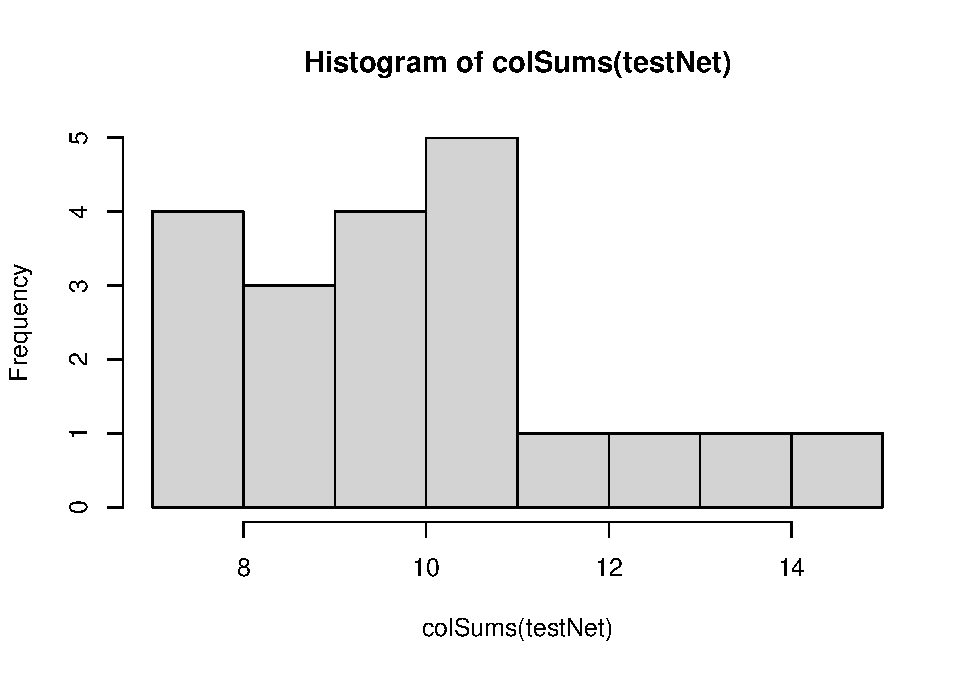
\includegraphics{20220404_miss_data_model_files/figure-latex/example with multiple predictors-1.pdf}

\begin{Shaded}
\begin{Highlighting}[]
\FunctionTok{mean}\NormalTok{(}\FunctionTok{colSums}\NormalTok{(testNet))}
\end{Highlighting}
\end{Shaded}

\begin{verbatim}
## [1] 10.3
\end{verbatim}

\begin{Shaded}
\begin{Highlighting}[]
\CommentTok{\# choosing some parameter values}
\NormalTok{alpha }\OtherTok{=} \SpecialCharTok{{-}}\DecValTok{5}
\NormalTok{beta }\OtherTok{=} \FunctionTok{c}\NormalTok{(}\FloatTok{0.05}\NormalTok{, }\FloatTok{0.23}\NormalTok{)}
\NormalTok{netStats }\OtherTok{=} \FunctionTok{data.frame}\NormalTok{(}\AttributeTok{degree =} \FunctionTok{degree}\NormalTok{(testNet), }\AttributeTok{indeg =} \FunctionTok{colSums}\NormalTok{(testNet))}

\CommentTok{\# make missing data indicator}
\NormalTok{missDatInd }\OtherTok{=} \FunctionTok{degradeNetLogis}\NormalTok{(}\AttributeTok{net =}\NormalTok{ testNet,}
                             \AttributeTok{alpha =}\NormalTok{ alpha,}
                             \AttributeTok{beta =}\NormalTok{ beta,}
                             \AttributeTok{netStats =}\NormalTok{ netStats,}
                             \AttributeTok{directed =} \ConstantTok{FALSE}\NormalTok{)}

\CommentTok{\# check total amount of missing ties after the adjmat adjustments, should be \textasciitilde{}80 (20\^{}2 * 0.2), maybe a bit less because of the adjmat adjustments}
\FunctionTok{sum}\NormalTok{(missDatInd)}
\end{Highlighting}
\end{Shaded}

\begin{verbatim}
## [1] 82
\end{verbatim}

\begin{Shaded}
\begin{Highlighting}[]
\CommentTok{\# and we deplete}
\NormalTok{degradedNetMNAR2 }\OtherTok{=}\NormalTok{ testNet}
\NormalTok{degradedNetMNAR2[missDatInd}\SpecialCharTok{==}\DecValTok{1}\NormalTok{] }\OtherTok{=} \ConstantTok{NA}

\CommentTok{\# plot side by side}
\FunctionTok{par}\NormalTok{(}\AttributeTok{mfrow =} \FunctionTok{c}\NormalTok{(}\DecValTok{1}\NormalTok{,}\DecValTok{2}\NormalTok{))}
\FunctionTok{gplot}\NormalTok{(testNet, }\AttributeTok{xlab =} \StringTok{"Toy net"}\NormalTok{, }\AttributeTok{gmode =} \StringTok{"graph"}\NormalTok{)}
\FunctionTok{gplot}\NormalTok{(degradedNetMNAR2, }\AttributeTok{xlab =} \StringTok{"MNAR degraded net"}\NormalTok{, }\AttributeTok{gmode =} \StringTok{"graph"}\NormalTok{)}
\end{Highlighting}
\end{Shaded}

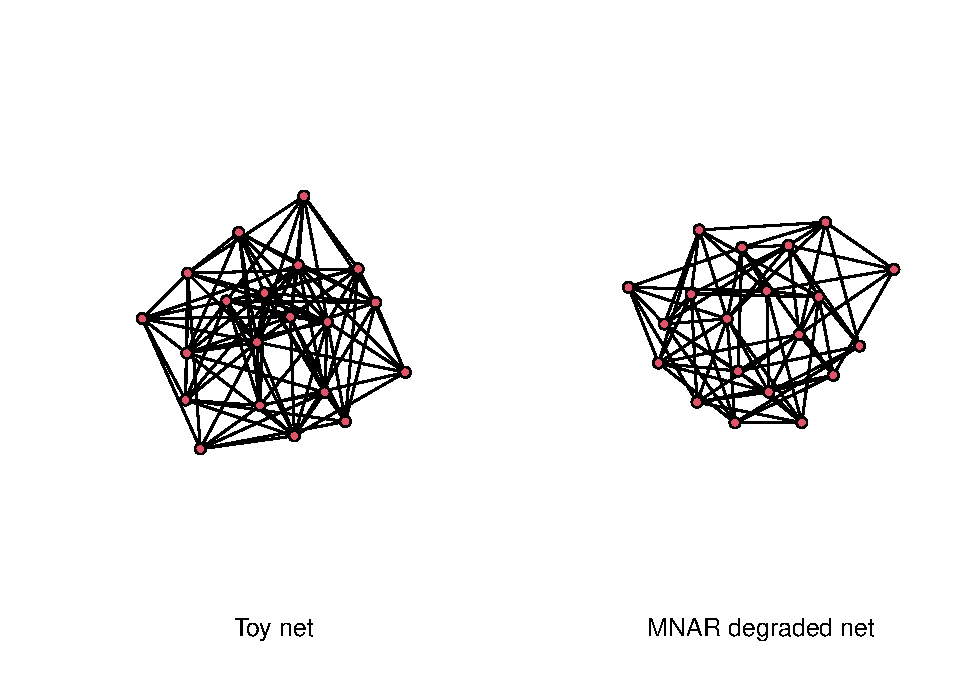
\includegraphics{20220404_miss_data_model_files/figure-latex/example with multiple predictors-2.pdf}

\begin{Shaded}
\begin{Highlighting}[]
\CommentTok{\# it\textquotesingle{}s quite hard to see, but if we see the average degree centrality and their histograms,}
\FunctionTok{hist}\NormalTok{(}\FunctionTok{degree}\NormalTok{(testNet), }\AttributeTok{main =} \FunctionTok{paste}\NormalTok{(}\StringTok{"Mean = "}\NormalTok{,}\FunctionTok{mean}\NormalTok{(}\FunctionTok{degree}\NormalTok{(testNet)), }\StringTok{" SD = "}\NormalTok{, }\FunctionTok{round}\NormalTok{(}\FunctionTok{sd}\NormalTok{(}\FunctionTok{degree}\NormalTok{(testNet)), }\DecValTok{2}\NormalTok{), }\AttributeTok{sep =} \StringTok{""}\NormalTok{))}
\FunctionTok{hist}\NormalTok{(}\FunctionTok{degree}\NormalTok{(degradedNetMNAR2), }\AttributeTok{main =} \FunctionTok{paste}\NormalTok{(}\StringTok{"Mean = "}\NormalTok{,}\FunctionTok{mean}\NormalTok{(}\FunctionTok{degree}\NormalTok{(degradedNetMNAR2)), }\StringTok{" SD = "}\NormalTok{, }\FunctionTok{round}\NormalTok{(}\FunctionTok{sd}\NormalTok{(}\FunctionTok{degree}\NormalTok{(degradedNetMNAR2)), }\DecValTok{2}\NormalTok{), }\AttributeTok{sep =} \StringTok{""}\NormalTok{))}
\end{Highlighting}
\end{Shaded}

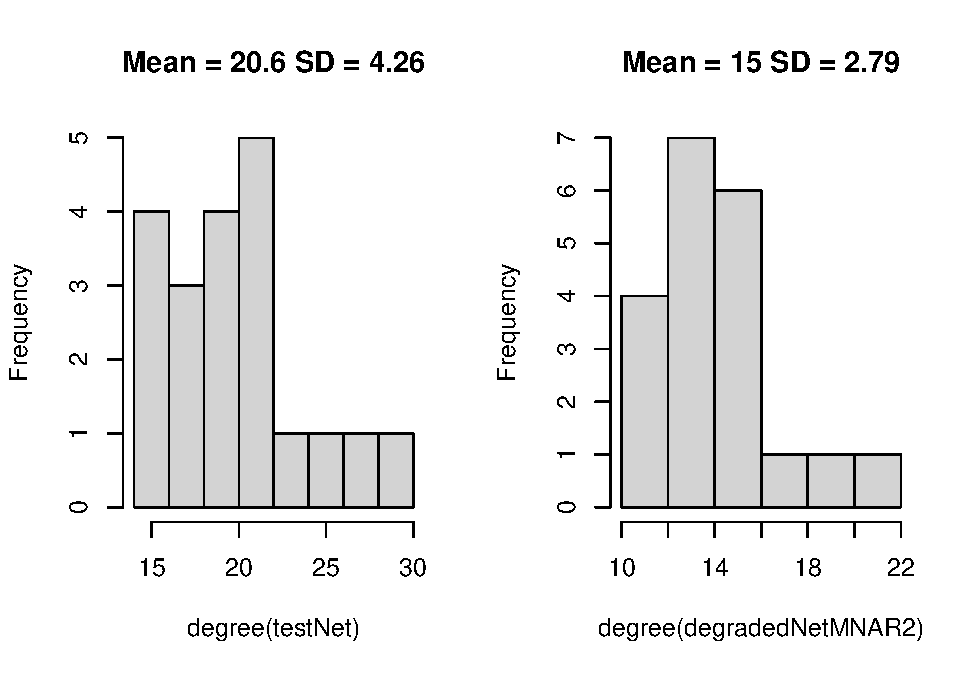
\includegraphics{20220404_miss_data_model_files/figure-latex/example with multiple predictors-3.pdf}

The model above can be thought of as:

\[\Pr(\mathbf{D}_{ij} = 1) = logistic(\alpha + \beta_1(\mathbf{X}_{i+} + \mathbf{X}_{+j}) + \beta_2(\mathbf{X}_{+j})),\]

and similar to the example before, if we wanted \textasciitilde20\%
missingness,

\[\frac{\sum_{i = 1..n} \frac{1}{1 + \exp(-\alpha - \beta_1(\mathbf{X}_{i+} + \mathbf{X}_{+j}) - \beta_2(\mathbf{X}_{+j}))}}{n} = 0.2.\]

After filling in the values with the test network (testNet), where the
mean degree is 20.6 (above), and the mean indegree is
\(\mathbf{\overline{X}}_{j+} = 10.3\)

\[\exp(-\alpha - 20.6\beta_1 - 10.3\beta_2) = 4,\]

\[-\alpha - 20.6\beta_1 - 10.3\beta_2= \log(4),\]

Don't exactly know how to solve this, I just kept guessing numbers to
get a mean of \textasciitilde0.2.

The model itself isn't particularly intuitive either, the higher the
degree (which counts indegree, so it's counted twice) and the higher the
indegree, the more likely a tie variable is to be missing. But the
important(?) part is that I can put multiple things in the model and
weigh certain aspects of the network more than other aspects (e.g., I
might think indegree matters more than the overall degree)

\begin{quote}
what can we do from here on?
\end{quote}

Two sides:

\begin{quote}
the modelling front (i.e., wrt to methods)
\end{quote}

The modelling front can be improved and extended in a lot of
ways\ldots{} Programming-wise, sensitivity plots where parameters scale
to missing data proportions would be nice (i.e., a fn to spit out
parameter values for a set proportion of missingness would be useful).
Undirected networks also need to acknowledge both ends (i.e., the
\(\beta\) model that's just a slightly modified Bernoulli model where we
may conceptualise it as the probability of a sender sending a tie with
the probability the receiver receives the tie.). We could always use
more complicated models, but I believe it's a better idea to neaten our
conceptual front before we make things more complex for the sake of
being complex.

Maybe there's something to do in the modelling front to disentangle the
missing data mechanism (\(\mathbf{D}\)) with whatever
decision-making-mechanism the network analyst is doing (similar to the
NSF false positive/miss rates?). This may be a meta perspective if we
were to account for differences in the way analysts approach the
collected resources to represent the network- that is that there may be
different ways for the `archaeological' approach to be done.

Would it be useful (or possible) to simulate how a covert network grows
over time from some semantically coded `data' (e.g., A is suspect, B is
connected to A by coarrests, C is A's non-illicit friend in legitimate
businesses), similar to how Pete made that gif of a network growing over
time, and then introducing missing data via a pre-specified mechanism?
This somehow sounds doable in my head, That being said, we're still
talking about unknown unknowns when we model MNAR missing data
mechanisms, so in terms of `how useful is this?', I don't really have a
clear answer.

Multiplexity, if we were to acknowledge covert networks as another type
of social network, they would have their own social dynamics in it and
so we may be able to represent valenced ties (e.g., position in the
hierarchy perhaps since actual data asking the covert actors how they
feel about other actors would be extremely unfeasible). Heterophily may
be another aspect to consider here in terms of roles in the covert
network. I feel like there's a lot of value in specifying types of
ties/relationships in elaborating particular network properties, but I
also think that this might grow to be very unfeasible in a ridiculous
pace if we wanted to \emph{really} describe multipartite nodes and/or
multiplex ties. Also, proximity (or physical distance). How do we deal
with that? Using some dodgy surveillance/data collection sources to
identify meetings? Maybe ethnographical measures are more sensible than
heavy computation semantic analysis solutions here?

\begin{quote}
the conceptual front (i.e., wrt to plausibility of the mechanisms)
\end{quote}

We can consider `popular' psych effects that replicate-ish to justify
the plausibility of some missing data mechanisms (e.g., the `bystander'
effect). Another think to think about is sampling frames for
investigators/detectives. How would two people approach and analyse a
covert network differently? Given n observers, perhaps the observers
systematically `sample' the network as a fn of `visibility' or whatever.
This would again be similar to having a model for missing data indicator
D that depends on characteristics of the network. However, the final
observed network(s) would be a product of many models for sampling and
actual missing mechanisms\ldots{} Is some kind of triangulation a
benefit of multiple network analysts' perspectives?

What do I need to brainstorm this? I'd love to know how `data' is
`collected'. What are the nuances that come up when we discuss missing
data mechanisms? Let alone from a data analyst's perspective, but from
the observed network's perspective as well. How important are brokers?
Spies? High-social-capital-actors? `Extreme' actors? This might just
result in a `betweenness' argument, but maybe something to look into is
the brokerage aspects in a conceptual front? I mean, assuming that the
actors will act in a way to optimise network efficiency with security,
the `ideal' position probably is being sparsely connected to
high-connected nodes. Sparsely connected to decrease visibility, but
connected to well-connected nodes so that this particular node has a lot
of `reach'. In that sense, would geodesic distance (or just generally
path lengths) be a useful metric? Or inverse average geodesic
(`efficiency'). I don't really think centralities are the be-all-end-all
in identifying potentially important actors in a network. In simple and
ideal cases sure, but when the network gets complicated (and maybe if
the `authority' is sparsely connected), centrality's usefulness goes
down real fast. Do we need abstract algebras for identifying roles now,
or is this something we can leave to data??

When acknowledging that the archaelogical approaches to `representing' a
network may differ, how exactly can they differ? Some analysts may have
resources that emphasise some nodes more than the other. There's also
the time element since investigations are cumulative efforts (i.e., only
more information can be gained through the passage of time). It would be
neat if we had \emph{something} to describe how a network evolves w.r.t.
the progress of an investigation (e.g., perhaps how prime suspects
change through time and how this matches up with whatever evidence is
recorded). Of course, one other thing is the politics (?) of the
situation. I'm assuming resources are limited, so investigations may be
ushered to `wrap up' and prosecute the prime suspect due to various
pressures (e.g., political, economical, etc.).

How does the `investigation' network grow? Is it via a snowball
mechanism? Surely informants play a role here to connect potential
covert actors\ldots{} If I were to imagine I were an analyst part of an
investigation collating information, I would simply just represent what
the most common threads in the evidence are if I were to `construct' a
network. I (the network analyst) feel like I would have no agency on
which possible ties I'd want to investigate since it would be somewhat
data-driven. Is it a collaborative effort with more than one analyst,
all of whom have different sources of information? Or is it usually done
under a central figure commanding the analysis like a head analyst?

Can the missing data mechanism `progress' over time as the investigation
proceeds as a response to the investigation? Some kind of defensive
mechanism for the covert network to reorganise itself in response to the
investigation? In that sense, would I need to acknowledge the missing
data mechanism to be a temporal process or from an `omniscient observer'
perspective where I assume I know the entire covert network? How would I
even acknowledge how a missing data mechanism can grow? The missingness
just gets snowballed?

What about using qualitative aspects of ties? If we knew that certain
actors in the covert network share antagonistic ties, would they be more
reliable informants? Given the scattered aspect of the `raw data',
multiplexity may be a boon in disguise if we wanted to identify
important actors or potential informants for further information. Point
is, in the most basic sense, `ties' can mean different things to
different actors and I don't see why this would be different for covert
networks (i.e., a covert network is still a network with its own
dynamics).

Do covert networks `grow' in the same way a non-covert network does in a
snowball sense?

How do we go about identifying `extreme actors' (i.e., `outliers' who
are incredibly influential in the network) beyond centrality? What kind
of structures would we want to try see? Perhaps path-length measures,
alternating n stars (though this would just be a degree
centrality\ldots)?

\end{document}
